\documentclass{article}

\usepackage[utf8]{inputenc}
\usepackage{graphicx}
\usepackage{amsmath}
\usepackage[letterpaper, portrait, margin=1in]{geometry}
\usepackage{gensymb}
\title{Molecules and Cells HW 5}
\date{September 29th, 2016}

\begin{document}

\maketitle

1. \begin{figure}[h]
  \centering
 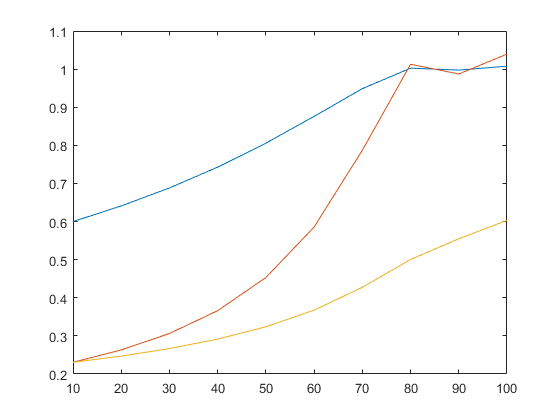
\includegraphics[scale=0.5]{P1.png}
\end{figure}
The light arrows represent the direction of DNA synthesization, and the black arrows represent the direction of movement for the bubble.

2a. The presence of small molecules would affect the $T_m$. DNA is a negative molecule due to the phosphate group. The salt molecules would help stabilize DNA, increasing $T_m$.

2b.	$T_m$ would increase with more C+G because these two nucleic acids bind with 3 hydrogen bonds rather than A+T's two, so more energy would be needed to break the bonds. $T_m$ also increases with length because there would be more bonds to break to make a longer chain separate.

2c. $T_m=59.9+0.41(50)-675/100=73.65\degree C$

3. (E) A=Arrival, P=Protein Elongation, E=Exit
\begin{figure}[h]
  \centering
 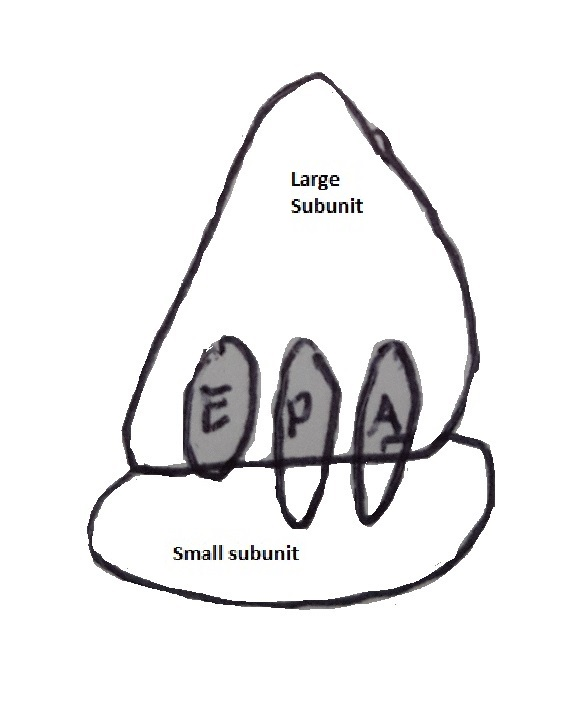
\includegraphics[scale=0.21]{P3.jpg}
\end{figure}

4a. quaternary structure

4b. $\alpha$-helix

4c. primary structure

4d. binding site

4e. polypeptide backbone

4f. $\beta$-sheet

4g. antibody

4h. allosteric protein

4i. gene

4j. antiparallel

4k. RNA primer

4l. ligase

4m. DNA helicase

4n. leading strand

4o. sliding clamp

4p. replication fork

4q. lagging strand
\vspace{5mm}

5. 3'-TACCACGTG-5' or 5'-GTGCACCAT-3'
\vspace{5mm}

6. 
\begin{figure}[h]
  \centering
 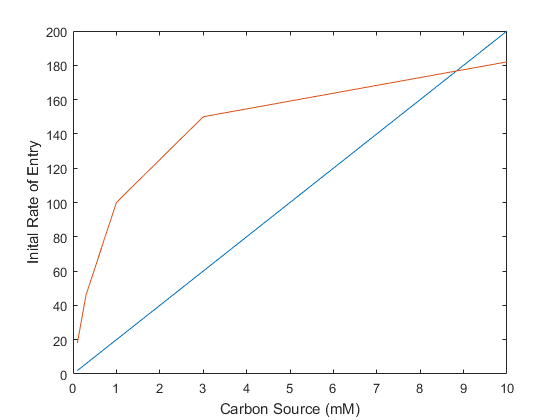
\includegraphics[scale=0.5]{P6.png}
\end{figure}

Synthesizes DNA in 5' to 3' direction

Error checking in 3' to 5' direction
\vspace{5mm}

7a. 3'-CCTAAAAACAGGTGTTAGT-5' or 5'-TGATTGTGGAGACAAAAATCC-3'

7b. Since complementary strands run in opposite directions, the phosphate group is on the 5' end.

7c. No, DNA replication copies over the complementary nucleotides. Because DNA does not have to be symmetrical, the new strand is not the same as the parental strand.
\vspace{5mm}

8. \begin{figure}[h]
  \centering
 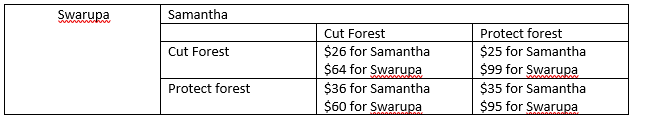
\includegraphics[scale=0.6]{P8.png}
\end{figure}

The sugar is a ribose.
\vspace{5mm}

9. The molar percent of G has to be the same as C, so it must be 30\%. Then, the remaining percentages must be split equally between A and T, so both of them must 20\%.
\vspace{5mm}

10. True,True
\vspace{5mm}

11. (E) There are 6 codons for Arg, 6 codons for Leu, and 6 codons for Ser, for a total of $6*6*6=216$ possibilities.
\vspace{5mm}

12. (D)
\vspace{5mm}

13a. \begin{figure}[h]
  \centering
 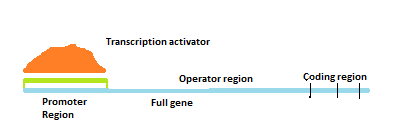
\includegraphics[scale=0.7]{P13.png}
\end{figure}

13b. The gene has 2 introns and 3 exons.
\vspace{5mm}

14. Since RNA polymerase transcribes from 3' to 5', the bottom strand is the template. The resulting RNA strand is 5'-GUAACGGAUG-3'
\end{document}